\chapter{Arhitektura i dizajn sustava}

		Arhitektura se može podijeliti na tri podsustava:
		\begin{itemize}
			\item 	Web poslužitelj
			\item 	Web aplikacija
			\item 	Baza podataka		
		\end{itemize}

		\underbar{Web preglednik} predstavlja softverski program koji omogućuje korisnicima 
		pregledavanje web-stranica i konzumiranje povezanih multimedijskih sadržaja. 
		Svaki internetski preglednik djeluje kao prevoditelj, interpretirajući kôd web 
		stranica napisan u određenom programskom jeziku i pretvarajući ga u vizualni 
		format razumljiv svakom korisniku. Drugim riječima, stranice su izvorno napisane 
		u kodu, a \textit{web preglednik} ih interpretira kako bi korisnicima pružio čitljiv i 
		interaktivan prikaz. Kada korisnik želi pristupiti određenoj web stranici, 
		šalje zahtjev \textit{web poslužitelju} putem \textit{web preglednika}, što pokreće proces 
		prijenosa informacija i omogućava korisnicima interakciju s odabranim sadržajem.


		\underbar{Web poslužitelj} temelj je rada web aplikacije. Zadužen je za komunikaciju
		klijenta sa aplikacijom. Međusobna komunikacija odvija se putem HTTP (engl. \textit{Hyper
		Text Transfer Protocol}) protokola, koji je jedan od protokola za prijenos informacija
		na webu.

		Korisnik koristi \textit{web aplikaciju} za obrađivanje željenih zahtjeva.
		\textit{Web aplikacija} gleda zahtjev te ovisno o njemu, pristupa bazi podataka nakon čega
		preko \textit{web poslužitelja} vraća korisniku odgovor u HTML dokumentu koji je 
		vidljiv u \textit{web pregledniku}.

		Programski jezik koji smo odabrali za izradu naše \textit{web aplikacije} je Java, zajedno
		sa Spring Boot radnim okvirom te programski jezik JavaScript zajedno sa React radnim okvirom.

		Ovisno o ulogama u timu, odabrana razvoja okruženja su:

		\begin{itemize}
			\item Frontend - Visual Studio Code
			\item Backend - Intellij IDEA
			\item Dokumentacija - Visual Studio Code		
		\end{itemize}

		Arhitekura sustava zasnivat će se na MVC (Model-View-Controller) konceptu.
		Spring Boot nudi veliku podršku za rad sa Spring MVC-om te kao takav
		odgovara našim zahtjevima (također olakšava konfiguraciju potrebnu za validan rad
		Spring MVC-a).

		MVC koncept omogućava nezavisan razvoj pojedinih dijelova aplikacije te kao takav
		olakšava ispitivanje, razvijanje i dodavanje novih svojstva u aplikaciju.

		\medbreak

		Temeljne komponente MVC koncepta su:
		\begin{itemize}
			\item Model - dinamičke strukture podataka, npr. entitet User, Ingredient...
			\item View - ono što korisnik vidi, vizualizacija podataka
			\item Controller - poveznica između Model-a i View-a, bavi se HTTP zahtjevima i odgovorima		
		\end{itemize}

		\eject
				
		\section{Baza podataka}

			U našem sustavu, koristit ćemo relaciju bazu podataka koja je strukturom prilagođena
			modeliranju stvarnog svijeta. Osnovna gradivna jedinka baze je relacija, tj. tablica
			koja je identificirana svojim imenom i skupom atributa. Glavna svrha baze podataka je
			brza i jednostavna pohrana, izmjena te dohvat podataka za određenu uporabu.

			\medbreak

			Upravitelj bazom podataka:
			\begin{itemize}
				\item PostgreSQL		
			\end{itemize}

			\medbreak

			Entiteti bazom podataka:
			\begin{itemize}
				\item users
				\item userFollow		
				\item chatMessage		
				\item communicationTime
				\item recipe		
				\item recipeRating		
				\item bookmarkedRecipe		
				\item role		
				\item category		
				\item tag		
				\item ingredient		
				\item cuisine		
				\item video		
				\item image		
				\item media				
			\end{itemize}
			
			\eject

			\subsection{Opis tablica}

				\textbf{users} Relacija pohranjuje entitete modela koji predstavlaju korisnika.
				Ograničenje stranog ključa odnosi se na atribut roleId koji označava id
				razine pristup (Klijent, Vlasnik, Admin) koju korisnik ima; referencirana je
				relacija role, stupac id. 
				
				\begin{longtblr}[
					label=none,
					entry=none
					]{
						width = \textwidth,
						colspec={|X[6,l]|X[6, l]|X[20, l]|}, 
						rowhead = 1,
					} %definicija širine tablice, širine stupaca, poravnanje i broja redaka naslova tablice
					\hline \SetCell[c=3]{c}{\textbf{users}}	 \\ \hline[3pt]
					\SetCell{LightGreen}id & INT	&  	jedinstveni identifikator korisnika  	\\ \hline
					firstName	& VARCHAR &   ime korisnika	\\ \hline 
					lastName & VARCHAR & prezime korisnika  \\ \hline 
					username & VARCHAR	&  korisničko ime korisnika		\\ \hline
					email & VARCHAR	&  adresa elektroničke pošte korisnika		\\ \hline
					password & VARCHAR	&  hash lozinke		\\ \hline 
					\SetCell{LightBlue} roleId	& VARCHAR &  identifikator razine pristupa korisnika (role.id) 	\\ \hline 
				\end{longtblr}

				\textbf{userFollow} Relacija pohranjuje entitete modela koji predstavlja odnos praćenja
				korisnika i autora.
				Ograničenje stranog ključa odnosi se na atribute followerId i authorId koji označavaju
				id korisnika koji je inicirao praćenje, tj. korisnika koji je autor recepta; referencirana je
				relacija users, stupac id.

				\begin{longtblr}[
					label=none,
					entry=none
					]{
						width = \textwidth,
						colspec={|X[6,l]|X[6, l]|X[20, l]|}, 
						rowhead = 1,
					} %definicija širine tablice, širine stupaca, poravnanje i broja redaka naslova tablice
					\hline \SetCell[c=3]{c}{\textbf{userFollow}}	 \\ \hline[3pt]
					\SetCell{LightGreen}id & INT	&  	jedinstveni identifikator modela praćenja	\\ \hline
					\SetCell{LightBlue} followerId	& INT &   id korisnika koji prati 	(user.id)\\ \hline 
					\SetCell{LightBlue} authorId & INT & id autora kojeg se prati  (user.id)\\ \hline 
					followedAt & TIMESTAMP	&  vrijeme početka praćenja		\\ \hline
				\end{longtblr}

				\textbf{chatMessage} Relacija pohranjuje entitete modela koji predstavlja
				poruke koje se koriste pri komunikaciji.
				Ograničenje stranog ključa odnosi se na atribute senderId i receiverId koji označavaju
				id korisnika koji je posalo poruku, tj. korisnika koji poruku treba primiti; referencirana je
				relacija users, stupac id.
				
				\begin{longtblr}[
					label=none,
					entry=none
					]{
						width = \textwidth,
						colspec={|X[6,l]|X[6, l]|X[20, l]|}, 
						rowhead = 1,
					} %definicija širine tablice, širine stupaca, poravnanje i broja redaka naslova tablice
					\hline \SetCell[c=3]{c}{\textbf{chatMessage}}	 \\ \hline[3pt]
					\SetCell{LightGreen}id & INT	&  	jedinstveni identifikator poruke (user.id)	\\ \hline
					\SetCell{LightBlue} senderId	& INT &  id pošiljatelja (user.id)  	\\ \hline 
					\SetCell{LightBlue} receiverId & INT & id primatelja (user.id) \\ \hline 
					content & VARCHAR	&  sadržaj poruke		\\ \hline
				\end{longtblr}

				\textbf{communicationTime} Relacija pohranjuje entitete modela koji predstavlja
				dostupnost korisnika za komunikaciju.
				Ograničenje stranog ključa odnosi se na atribut userId koji označava
				id korisnika koji prikazuje vrijeme u koje je dostupan za komunikaciju; referencirana je
				relacija users, stupac id.

				\begin{longtblr}[
					label=none,
					entry=none
					]{
						width = \textwidth,
						colspec={|X[6,l]|X[6, l]|X[20, l]|}, 
						rowhead = 1,
					} %definicija širine tablice, širine stupaca, poravnanje i broja redaka naslova tablice
					\hline \SetCell[c=3]{c}{\textbf{communicationTime}}	 \\ \hline[3pt]
					\SetCell{LightGreen}id & INT	&  	jedinstveni identifikator \\ \hline
					\SetCell{LightGreen}userId	& INT &   jedinstveni identifikator korisnika (user.id)\\ \hline 
					\SetCell{LightGreen}start & TIMESTAMP & vrijeme od  \\ \hline 
					\SetCell{LightGreen}end & TIMESTAMP	&  vrijeme do		\\ \hline
				\end{longtblr}

				\textbf{recipe} Relacija pohranjuje entitete modela recept.
				Ograničenje stranog ključa odnosi se na atribute ingredientId, tagId, categoryId, cuisineId, mediaId
				te userId koji označavaju, redom, sastojke recepta, oznake recepta, kategoriju u koju recept spada,
				kuhinju u koju recept spada, multimedijske sadržaje koje recept sadrži te autora recepta.
				Relacije koje se referenciraju su, redom, ingredient (stupac id), tag (stupac id), category (stupac id),
				cuisine (stupac id), media (stupac id), user (stupac id). 
				
				Zbog jednostavnosti vizualnog prikaza, odnosi @ManyToMany nisu prikazani zasebnom relacijom.
				
				Redom:
				\begin{itemize}
					\item 	N:N sa ingredient
					\item 	N:N sa tag
					\item 	N:N sa media	
				\end{itemize}

				\begin{longtblr}[
					label=none,
					entry=none
					]{
						width = \textwidth,
						colspec={|X[6,l]|X[6, l]|X[20, l]|}, 
						rowhead = 1,
					} %definicija širine tablice, širine stupaca, poravnanje i broja redaka naslova tablice
					\hline \SetCell[c=3]{c}{\textbf{recipe}}	 \\ \hline[3pt]
					\SetCell{LightGreen}id & INT	&  	jedinstveni identifikator recepta  	\\ \hline
					\SetCell{LightBlue} ingredientId	& INT &   id sastojka 	(ingredient.id)\\ \hline 
					\SetCell{LightBlue} tagId	& INT &   id oznake	(tag.id)\\ \hline 
					\SetCell{LightBlue} categoryId	& INT &   id kategorije	(category.id)\\ \hline 
					\SetCell{LightBlue} cuisineId & INT & id zemlje podrijetla (cuisine.id) \\ \hline 
					\SetCell{LightBlue} mediaId & INT & id multimedijske stavke (media.id) \\ \hline 
					\SetCell{LightBlue} userId & INT	&  id autora (user.id)	\\ \hline
					title & VARCHAR	&  naslov recepta		\\ \hline
					description & VARCHAR	& opis recepta		\\ \hline 
					cookingTime	& INTERVAL &  vrijeme kuhanja 	\\ \hline 
				\end{longtblr}

				\textbf{recipeRating} Relacija pohranjuje modele entiteta koji predstavljaju
				\textit{feedback} na recept; ocjenu i komentar.
				Ograničenje stranog ključa odnosi se na atribute userId i recipeId koji označavaju
				id korisnika koji daje \textit{feedback} i recept koji se komentira; referencirana je
				relacija users, stupac id te relacija recipe, stupac id.

				\begin{longtblr}[
					label=none,
					entry=none
					]{
						width = \textwidth,
						colspec={|X[6,l]|X[6, l]|X[20, l]|}, 
						rowhead = 1,
					} %definicija širine tablice, širine stupaca, poravnanje i broja redaka naslova tablice
					\hline \SetCell[c=3]{c}{\textbf{recipeRating}}	 \\ \hline[3pt]
					\SetCell{LightGreen}id & INT	&  	jedinstveni identifikator ocjene  	\\ \hline
					\SetCell{LightBlue} userId & INT	&  id klijenta koji je dao ocjenu (user.id)	\\ \hline 
					\SetCell{LightBlue} recipeId & INT & id recepta (recipe.id) \\ \hline 
					rating& INT	&  ocjena	\\ \hline
					comment & VARCHAR	&  komentar		\\ \hline
					createdAt & TIMESTAMP	& vrijeme nastanka ocjene		\\ \hline  
				\end{longtblr}

				\textbf{bookmarkedRecipe} Relacija pohranjuje model entiteta koji predstavlja zabilježbu recepta
				od strane nekog korisnika.
				Ograničenje stranog ključa odnosi se na atribute userId i recipeId koji označavaju
				id korisnika koji zabilježuje recept te id recepta koji se zabilježuje; referencirana je
				relacija users, stupac id te relacija recipe, stupac id.

				\begin{longtblr}[
					label=none,
					entry=none
					]{
						width = \textwidth,
						colspec={|X[6,l]|X[6, l]|X[20, l]|}, 
						rowhead = 1,
					} %definicija širine tablice, širine stupaca, poravnanje i broja redaka naslova tablice
					\hline \SetCell[c=3]{c}{\textbf{bookmarkedRecipe}}	 \\ \hline[3pt]
					\SetCell{LightGreen}id & INT	&  	jedinstveni identifikator zabilježbe recepta  	\\ \hline
					\SetCell{LightBlue} userId & INT	&  id klijenta koji je dao ocjenu (user.id)	\\ \hline 
					\SetCell{LightBlue} recipeId & INT & id recepta (recipe.id) \\ \hline 
					createdAt & TIMESTAMP	& vrijeme nastanka ocjene		\\ \hline  
				\end{longtblr}

				\textbf{role} Relacija pohranjuje model entiteta koji predstavlja
				"ulogu", tj. razinu prava pristupa korisnika (Klijent, Vlasnik, Autor).

				\begin{longtblr}[
					label=none,
					entry=none
					]{
						width = \textwidth,
						colspec={|X[6,l]|X[6, l]|X[20, l]|}, 
						rowhead = 1,
					} %definicija širine tablice, širine stupaca, poravnanje i broja redaka naslova tablice
					\hline \SetCell[c=3]{c}{\textbf{role}}	 \\ \hline[3pt]
					\SetCell{LightGreen}id & INT	&  	jedinstveni identifikator razine pristupa\\ \hline
					name	& VARCHAR &  ime razine pristupa  	\\ \hline 
				\end{longtblr}

				\textbf{category} Relacija pohranjuje model entiteta koji predstavlja
				kategoriju u koju recept može pripadati.

				\begin{longtblr}[
					label=none,
					entry=none
					]{
						width = \textwidth,
						colspec={|X[6,l]|X[6, l]|X[20, l]|}, 
						rowhead = 1,
					} %definicija širine tablice, širine stupaca, poravnanje i broja redaka naslova tablice
					\hline \SetCell[c=3]{c}{\textbf{category}}	 \\ \hline[3pt]
					\SetCell{LightGreen}id & INT	&  	jedinstveni identifikator kategorije\\ \hline
					name	& VARCHAR &  ime kategorije  	\\ \hline 
				\end{longtblr}

				\textbf{tag} Relacija pohranjuje model entiteta koji predstavlja
				oznaku koji recept može imati (npr. Vegan, Healthy, Quick...)
				
				\begin{longtblr}[
					label=none,
					entry=none
					]{
						width = \textwidth,
						colspec={|X[6,l]|X[6, l]|X[20, l]|}, 
						rowhead = 1,
					} %definicija širine tablice, širine stupaca, poravnanje i broja redaka naslova tablice
					\hline \SetCell[c=3]{c}{\textbf{tag}}	 \\ \hline[3pt]
					\SetCell{LightGreen}id & INT	&  	jedinstveni identifikator oznake recepta\\ \hline
					name	& VARCHAR &  opis oznake recepta  	\\ \hline 
				\end{longtblr}

				\textbf{ingredient} Relacija pohranjuje model entiteta koji predstavlja
				sastojak koji recept može sadržavati.

				\begin{longtblr}[
					label=none,
					entry=none
					]{
						width = \textwidth,
						colspec={|X[6,l]|X[6, l]|X[20, l]|}, 
						rowhead = 1,
					} %definicija širine tablice, širine stupaca, poravnanje i broja redaka naslova tablice
					\hline \SetCell[c=3]{c}{\textbf{ingredient}}	 \\ \hline[3pt]
					\SetCell{LightGreen}id & INT	&  	jedinstveni identifikator sastojka\\ \hline
					name	& VARCHAR &  ime sastojka  	\\ \hline 
				\end{longtblr}

				\textbf{cuisine} Relacija pohranjuje model entiteta koji predstavlja
				zemlju podrijetla recepta, tj. kuhinju iz koje recept potječe.

				\begin{longtblr}[
					label=none,
					entry=none
					]{
						width = \textwidth,
						colspec={|X[6,l]|X[6, l]|X[20, l]|}, 
						rowhead = 1,
					} %definicija širine tablice, širine stupaca, poravnanje i broja redaka naslova tablice
					\hline \SetCell[c=3]{c}{\textbf{cuisine}}	 \\ \hline[3pt]
					\SetCell{LightGreen}id & INT	&  	jedinstveni identifikator zemlje kuhanja\\ \hline
					name	& VARCHAR &  ime zemlje kuhanja  	\\ \hline 
				\end{longtblr}

				\textbf{video} Relacija pohranjuje model entiteta koji predstavlja
				medijski zapis oblika videa.

				\begin{longtblr}[
					label=none,
					entry=none
					]{
						width = \textwidth,
						colspec={|X[6,l]|X[6, l]|X[20, l]|}, 
						rowhead = 1,
					} %definicija širine tablice, širine stupaca, poravnanje i broja redaka naslova tablice
					\hline \SetCell[c=3]{c}{\textbf{video}}	 \\ \hline[3pt]
					\SetCell{LightGreen}id & INT	&  	jedinstveni identifikator videa\\ \hline
					duration	& INTERVAL &  trajanje videa  	\\ \hline 
				\end{longtblr}

				\textbf{image} Reliacija pohranjuje model entiteta koji predstavlja
				medijski zapis oblika fotografije.

				\begin{longtblr}[
					label=none,
					entry=none
					]{
						width = \textwidth,
						colspec={|X[6,l]|X[6, l]|X[20, l]|}, 
						rowhead = 1,
					} %definicija širine tablice, širine stupaca, poravnanje i broja redaka naslova tablice
					\hline \SetCell[c=3]{c}{\textbf{image}}	 \\ \hline[3pt]
					\SetCell{LightGreen}id & INT	&  	jedinstveni identifikator fotografije\\ \hline
					width	& INT &  širina fotografije (px)  	\\ \hline
					height	& INT &  visina fotografije (px)  	\\ \hline
					format  & VARCHAR & format fotografije \\ \hline
				\end{longtblr}
				
				\eject

				\textbf{media} Relacija pohranjuje model entiteta koji predstavlja medijski sadržaj
				koji je objavio neki korisnik, uz neki recept.
				Ograničenje stranog ključa odnosi se na atribute recipeId 
				id recepta uz okji je medijski sadržaj postavljen; referencirana je
				relacija recipe, stupac id.

				Medijska stavka može biti ili slika ili video.

				\begin{longtblr}[
					label=none,
					entry=none
					]{
						width = \textwidth,
						colspec={|X[6,l]|X[6, l]|X[20, l]|}, 
						rowhead = 1,
					} %definicija širine tablice, širine stupaca, poravnanje i broja redaka naslova tablice
					\hline \SetCell[c=3]{c}{\textbf{media}}	 \\ \hline[3pt]
					\SetCell{LightGreen}id & INT	&  	jedinstveni identifikator multimedijske stavke\\ \hline
					\SetCell{LightBlue}recipeId	& INT &  id recepta (px)  	\\ \hline
					key	& VARCHAR &   	naziv datoteke na oblaku\\ \hline
					description  & VARCHAR & opis multimedijske stavke \\ \hline
					uploadDate  & DATE & datum postavljanje multimedijske stavke \\ \hline

				\end{longtblr}
				
				\eject

				
				
			
			\subsection{Dijagram baze podataka}

			\begin{figure}[H]
				\rotatebox{90}{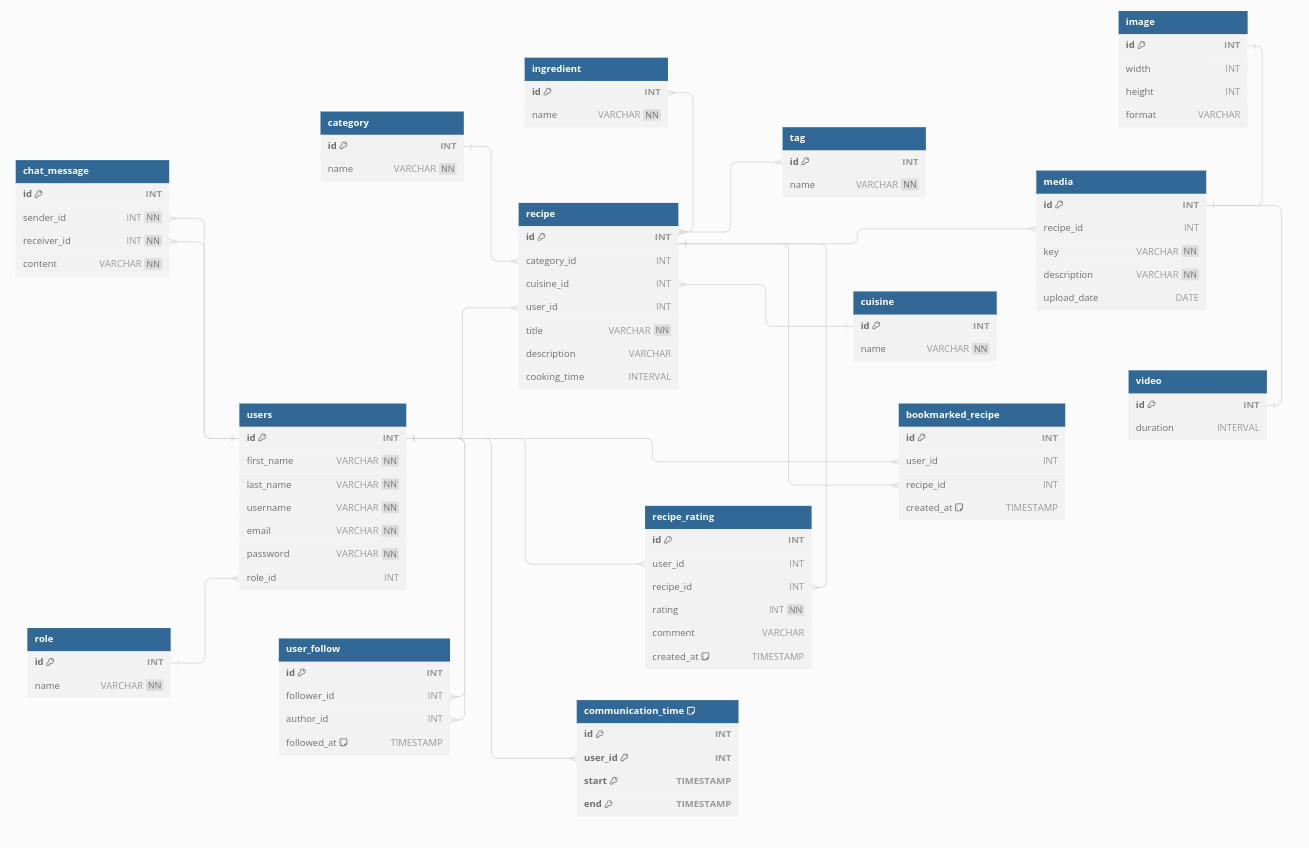
\includegraphics[scale=0.45]{slike/dijagram_baze.png}} 
				\centering
				\caption{Dijagram baze podataka}
				\label{fig:bpdiag}
			\end{figure}
			
			
			\eject
			
			
		\section{Dijagram razreda}
		
			\textit{Potrebno je priložiti dijagram razreda s pripadajućim opisom. Zbog preglednosti je moguće dijagram razlomiti na više njih, ali moraju biti grupirani prema sličnim razinama apstrakcije i srodnim funkcionalnostima.}\\
			
			\textbf{\textit{dio 1. revizije}}\\
			
			\textit{Prilikom prve predaje projekta, potrebno je priložiti potpuno razrađen dijagram razreda vezan uz \textbf{generičku funkcionalnost} sustava. Ostale funkcionalnosti trebaju biti idejno razrađene u dijagramu sa sljedećim komponentama: nazivi razreda, nazivi metoda i vrste pristupa metodama (npr. javni, zaštićeni), nazivi atributa razreda, veze i odnosi između razreda.}\\
			
			\textbf{\textit{dio 2. revizije}}\\			
			
			\textit{Prilikom druge predaje projekta dijagram razreda i opisi moraju odgovarati stvarnom stanju implementacije}
			
			
			
			\eject
		
		\section{Dijagram stanja}
			
			
			\textbf{\textit{dio 2. revizije}}\\
			
			\textit{Potrebno je priložiti dijagram stanja i opisati ga. Dovoljan je jedan dijagram stanja koji prikazuje \textbf{značajan dio funkcionalnosti} sustava. Na primjer, stanja korisničkog sučelja i tijek korištenja neke ključne funkcionalnosti jesu značajan dio sustava, a registracija i prijava nisu. }
			
			
			\eject 
		
		\section{Dijagram aktivnosti}
			
			\textbf{\textit{dio 2. revizije}}\\
			
			 \textit{Potrebno je priložiti dijagram aktivnosti s pripadajućim opisom. Dijagram aktivnosti treba prikazivati značajan dio sustava.}
			
			\eject
		\section{Dijagram komponenti}
		
			\textbf{\textit{dio 2. revizije}}\\
		
			 \textit{Potrebno je priložiti dijagram komponenti s pripadajućim opisom. Dijagram komponenti treba prikazivati strukturu cijele aplikacije.}